\documentclass[a4paper]{article}
\usepackage[UTF8]{ctex}
\usepackage{tikz}
\usepackage{xcolor}
\usepackage{amsmath}
\usepackage{amsthm}
\usepackage{amssymb}
\usepackage{enumerate}
\usepackage{float}
\usepackage{arydshln}
\usepackage{listingsutf8}
\usepackage{listings-ext}
\usepackage[margin=1in]{geometry}
% https://www.latexstudio.net/archives/9774.html
% https://www.latexstudio.net/archives/2234
% https://texample.net/

\lstset{
    basicstyle=\tt,
    keywordstyle=\color{purple}\bfseries,
    identifierstyle=\color{brown!80!black},
    commentstyle=\color{gray}
    showstringspaces=false,
}

\newtheorem{theorem}{\indent 定理}[section]
\newtheorem{lemma}[theorem]{\indent 引理}
\newtheorem{proposition}[theorem]{\indent 命题}
\newtheorem{corollary}[theorem]{\indent 推论}
\newtheorem{definition}{\indent 定义}[section]
\newtheorem{example}{\indent 例}[section]
\newtheorem{remark}{\indent 注}[section]
\newenvironment{solution}{\begin{proof}[\indent\bf 解]}{\end{proof}}
\renewcommand{\proofname}{\indent\bf 证明}

\tikzset{eaxis/.style={->,>=stealth}}

\title{组合优化与凸优化作业1}

\author{Homodeluna}
\date{2025 年 3 月 20 日}

\begin{document}
\maketitle
\section{}
设$S_1$,$S_2$是凸集,试讨论下列集合是否是凸集.
\begin{enumerate}
    \item $S_1 \cap S_2$
    \item $S_1 + S_2 = \{x+y | x \in S_1, y\in S_2\}$
    \item $S_1 - S_2 = \{x-y | x \in S_1, y\in S_2\}$
\end{enumerate}

\paragraph{解}
$S_1 \cap S_2$ 不是凸集

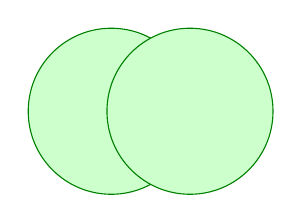
\begin{tikzpicture}
    \filldraw [fill=green!20!white, draw=green!50!black] (0,0) circle (30pt);
    \filldraw [fill=green!20!white, draw=green!50!black] (1,0) circle (30pt);
\end{tikzpicture}

$S_1 + S_2 = \{x+y | x \in S_1, y\in S_2\}$ 是凸集, 对于$p_1 = x_1 + y_1$ , $p_2 = x_2 + y_2$,
它们,的任一线性组合 $ap_1 + (1-a)p_2 \quad (0 \leq a \leq 1)$ 都可以分解为 $x_3 + y_3$,其中 $x_3 = ax_1 + (1-a)x_2$, $y_3 = ay_1 + (1-a)y_2$,而 $x_3 \in S_1. y_3 \in S_2$.

$S_1 + S_2 = \{x_y | x \in S_1, y\in S_2\}$ 是凸集,,证明方法与(b)类似.


\section{}

解释下列集合是否是凸集,为什么?
\begin{enumerate}
    \item $S = \{x | x_1^2 + x_2^2 \geq 4, 2 x_1 + x_2 \leq 10, -x_1 - x_2 \leq -10 x_2\}$
    \item $S = \{x | x_1 + x_2 \leq 6, -2 x_1 + 3x_2 \geq 2, 4x_1 - x_2 \leq 12 x_2\}$
    \item $S = \{x | -(x_1 -1)^2 + x_2 \geq 1,  x_1 + x_2 \geq 3, x_1 \geq 1\}$
    \item $S = \{x | x^2 \geq 1\}$
\end{enumerate}

1 不是

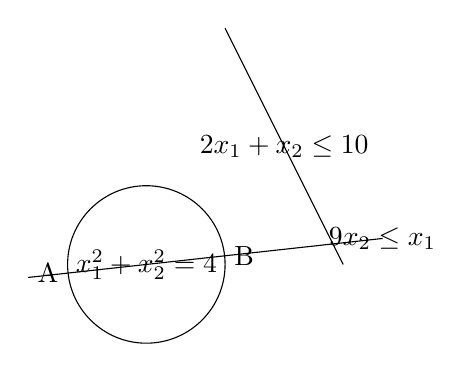
\begin{tikzpicture}[scale=0.5]
    \draw (0,0) circle (2) node {$x_1^2 + x_2^2 = 4$};
    \draw (5,0) -- node {$2 x_1 + x_2 \leq 10$} (2,6);
    \draw  (-3,-0.33) -- (6,0.66) node{$9x_2 \leq x_1$} ;
    \fill (-1.987,-0.221) node[left] {A};
    \fill (1.987,0.221) node[right] {B};
\end{tikzpicture}

取圆 $x_1^2 + x_2^2 = 4$ 与 直线 $9x_2 = x_1$ 的交点 $A  = (-9\sqrt{\frac{2}{41}},-\sqrt{\frac{2}{41}})$, $B = (9\sqrt{\frac{2}{41}},\sqrt{\frac{2}{41}})$, A和B都在集合内, 但是线段AB上的其他点(如(0,0))不在几何内,因此它不是凸集.

2 是 ,因为 $x_1 + x_2 \leq 6$ , $-2 x_1 + 3x_2 \geq 2$ , $4x_1 - x_2 \leq 12 x_2$三个集合都是凸集,它们的交也是凸集

3 是 $\{-(x_1 -1)^2 + x_2 \geq 1\}$ 是抛物线 $ x_2 = 1 + (x_1 - 1)^2$的上半叶,是凸集, $x_1 + x_2 \geq 3$ 和 $x_1 \geq 1$ 形状为半平面, 是凸集. 凸集的交集也是凸集.

4 不是. 该集合化简为 $(\infty,-1] \cap [1,\infty)$, 选定直线,$[-1,1]$,其中有直线上的点不在集合内(如0).


\section{}
设$f_1(x)$,$f_2(x)$,$f_3(x)$, ... $f_m(x)$均为凸函数,讨论下列函数是否是凸函数。若是则给出证明,否则举一反例。

\begin{enumerate}
    \item $g(x) = \max \{f_1(x), f_2(x), f_3(x) , ... , f_m(x)\} , \quad x \in \mathbb{R}$
    \item $g(x) = \min \{f_1(x), f_2(x), f_3(x) , ... , f_m(x)\} , \quad x \in \mathbb{R}$
    \item $g(x) = \sum_{i=1}^{n} x_i \log(x_i),\quad x \in \mathbb{R}^n, x_i > 0, \sum_{i=1}^n x_i = 1$
    \item $g(x) = \left\lfloor x \right\rfloor = \max\{k \leq x, k \text{是整数}\}$
    \item $g(x) = \sum_{i=1}^{k} x_{(i)}, \quad x \in \mathbb{R}^n , k \in \mathbb{Z}, 1 \leq k \leq n $, $x_{(i)}$ 表示向量x的第i个最大元素.
    \item $g(x) = x^2$
\end{enumerate}

1 是. 先证一个引理: 

\begin{lemma}
两个凸函数$f_1(x) : \mathbb{R} \rightarrow \mathbb{R}$ 和 $f_2(x): \mathbb{R} \rightarrow \mathbb{R}$,那么 $g(x) = \max \{f_1(x),f_2(x)\}$ 也是凸函数.
\end{lemma} 

\begin{proof}
对于点 x和y,取$z = \alpha x + (1-\alpha y)$,那么x,y,z 三点至少有两个点落到$f_1$和$f_2$中的一个上(如果三者都在同一个函数那么引理成立).

设 $g(x) = f_1(x)$, $g(z) = f_1(z)$, $g(y) = f_2(y)$,那么在y点 $g(y) = f_2(y) \geq f_1(y)$. 于是有:
\[
\begin{aligned}
     \alpha g(x) + (1-\alpha) g(y)  & =   \alpha f_1(x) + (1-\alpha) f_2(y) \\
   & \geq   \alpha f_1(x) + (1-\alpha) f_1(y)\quad (f_2(y) \geq f_1(y)) \\
   & \geq  f_1(z)  \\
    &=   g(z) 
\end{aligned}
\]

\end{proof}


然后考虑原问题,给定x,y,考虑 $\{ p | p = \alpha x + (1-\alpha)y, 0\leq \alpha \leq 1\}$这一子空间,其上有有限多段分段函数,逐一使用定理,即可证明$g(x)$在该子空间内是凸的.

2 不是. 考虑两个抛物线 $y = (x+3)(x+1)$和 $y = (x+3)(x+1)$, $g(x)$如下:

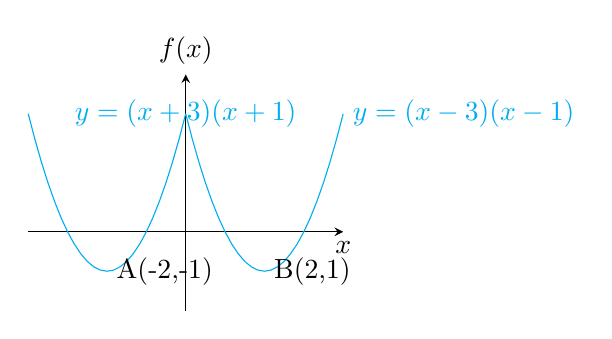
\begin{tikzpicture}[scale=0.5]
    \draw[eaxis] (-4,0) -- (4,0) node[below] {$x$};
    \draw[eaxis] (0,-2) -- (0,4) node[above] {$f(x)$};
    \draw [domain=-4:0, cyan] plot (\x,{(\x+1)*(\x+3)}) node {$y = (x+3)(x+1)$};
    \draw [domain=0:4, cyan] plot (\x,{(\x-1)*(\x-3)}) node[right] {$y = (x-3)(x-1)$};
    \fill (-2,-1) node[right] {A(-2,-1)};
    \fill (2,-1) node[right] {B(2,1)};
\end{tikzpicture}

它在AB段非凸. 

3 是.

给定 $x = (x_1,x_2 , ... x_n)$, $y = (y_1,y_2,...,y_n)$, 给定 $\alpha \in (0,1)$,那么考虑 $h(\alpha) = \sum_{i=1}^n (\alpha x_i + (1-\alpha) y_i) \ln (\alpha x_i + (1-\alpha) y_i)$ 

有
\[h'(\alpha) = \sum_{i=1}^n (x_i - y_i) \ln (\alpha x_i + (1-\alpha) y_i)\]
\[h''(\alpha) = \sum_{i=1}^n \frac{(x_i - y_i)^2} {\alpha x_i + (1-\alpha) y_i} \leq 0\]

因此 $h(\alpha)$是凸函数,有, 由$\alpha h(0) + (1-\alpha) h(1) \geq h(\alpha)$ 得 $\alpha g(x) +(a-\alpha)g(y) \geq g(\alpha x + (1-\alpha) y)$



4 不是, 考虑 $A=(0.5,0), B = (1.5,1),C = (1,0.5)$,可知ABC在同一线段上,该线段为$l(x)= x - 0.5$. 在$0.5 \leq x < 1$时有 $f(x) <= l(x)$,然而在 $1 \leq x \leq 1.5$时有 $f(x) \geq l(x)$.

5 是. 考虑辅助函数 $h_i(x)$,表示向量中的第i个最大元素.它对向量中的每一个分量都是凸的.证明方法与引理1类似.

$g(x) = \sum_{i=1}^k h_i(x)$,因此也是凸的.

6 是.  $g''(x) = 2 > 0$

\section{}
将下列线性规划问题化成标准型,并采用代数法,求解其所有的基本解,验证其最优解。  

\begin{enumerate}[a)]
    \item Min $z = 2x_1 - x_2 + 2x_3, s.t. \left\{ \begin{aligned}
        -x_1 + x_2 + x_3 = 4 \\
        -x_1 + x_2 - x_3 \leq 6\\
        x_1 \leq 0, x_2 \geq 0
    \end{aligned}\right.$
    \item Min $z = 2x_1 + x_2 + 3x_3 + x_4. s.t \left\{\begin{aligned}
        x_1 + x_2 + x_3 + x_4 \leq 7 \\
        2x_1 - 3x_2 + 5x_3 = -8\\
        x_1 - 2x_3 + 2x_4 \geq 1 \\
        x_1,x_3 \geq 0, x_2 \geq 0
    \end{aligned}\right.$
\end{enumerate}

\paragraph{a}
不等式化等式:

Min \(z=2x_1-x_2+2x_3 , s.t. \left\{\begin{aligned}
  -x_1+x_2+x_3=4 \\
  -x_1+x_2-x_3+x_4=6 \\
x_1 \leq 0,x_2 \geq 0,x_4 \geq 0
\end{aligned}\right.\)

去除无界变量:

Min \(z=2x_1-x_2+2x_3-2x_5 , s.t. \left\{\begin{aligned}
  -x_1+x_2+x_3-x_5=4 \\
  -x_1+x_2-x_3+x_4+x_5=6 \\
x_1 \leq 0,x_2 \geq 0,x_3 \geq 0,x_4 \geq 0,x_5 \geq 0
\end{aligned}\right.\)

去除负约束变量:

Min \(z=-2x_1-x_2+2x_3-2x_5 , s.t. \left\{\begin{aligned}
  x_1+x_2+x_3-x_5=4 \\
  x_1+x_2-x_3+x_4+x_5=6 \\
x_1  ... x_5 \geq 0
\end{aligned}\right.\)


上述方程消去$x_3$(使用$-2x_3 + x_4 = 2$), 得到 $2x_1 + x_2 + x_4 = 6$,这时方程的基本解,加上$x_1,x_2,x_4 \geq 0$的限制条件后得到基本可行解.

又 $z = -2x_1 - x_2 + 2x_3 = -2x_1 - x_2 + x_4 + 2$,最优解为\(\{x_1 = 0,x_2 = 3,x_4 = 0,x_3 = \frac{1}{2}\}\),此时$z=-2$
\paragraph{b}


4-2:
不等式化等式:

Min \(z=2x_1+x_2+3x_3+x_4 , s.t. \left\{\begin{aligned}
  x_1+x_2+x_3+x_4+x_5=7 \\
  2x_1-3x_2+5x_3=-8 \\
  x_1-2x_3+2x_4-x_6=-1 \\
x_1 \geq 0,x_2 \leq 0,x_3 , x5 ,x_6 \geq 0
\end{aligned}\right.\)

去除无界变量:

Min \(z=2x_1+x_2+3x_3+x_4-x_7 , s.t. \left\{\begin{aligned}
  x_1+x_2+x_3+x_4+x_5-x_7=7 \\
  2x_1-3x_2+5x_3=-8 \\
  x_1-2x_3+2x_4-x_6-2x_7=-1 \\
x_1 \geq 0,x_2 \leq 0,x_3...x_7 \geq 0
\end{aligned}\right.\)

去除负约束变量:

Min \(z=2x_1-x_2+3x_3+x_4-x_7 , s.t. \left\{\begin{aligned}
  x_1-x_2+x_3+x_4+x_5-x_7=7 \\
  2x_1+3x_2+5x_3=-8 \\
  x_1-2x_3+2x_4-x_6-2x_7=-1 \\
x_1 ... x_7 \geq 0
\end{aligned}\right.\)

%% TODO: 可行解,最优解

\section{}

用图解法解以下线性规划问题:
\begin{enumerate}[a)]
    \item Max $z = 3x_1 - 2x_2  s.t. \left\{ \begin{aligned}
        x_1 + x_2 \leq 4 \\
        x_1 + 2x_2 \geq 4\\
        x_1 , x_2 \geq 0
    \end{aligned}\right.$
    \item Min $f = -x_1 + 3x_2  s.t. \left\{ \begin{aligned}
        4x_1 + 7x_2 \geq 56 \\
        3x_1 + -5x_2 \geq 15\\
        x_1 , x_2 \geq 0
    \end{aligned}\right.$
\end{enumerate}

\paragraph{a} 无解
\begin{figure}[H]
    \centering
    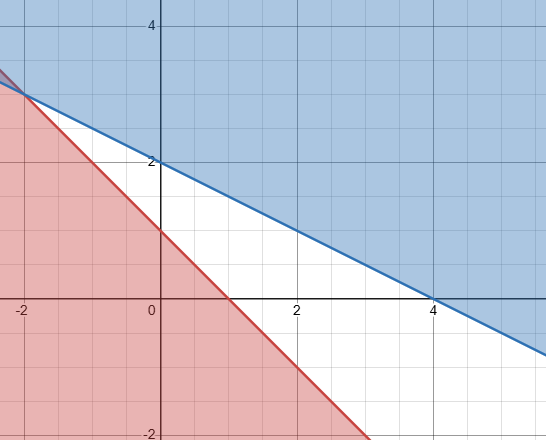
\includegraphics[width=0.7\textwidth]{pic/5-a.png}
\end{figure}

\paragraph{b}

根据观察可行域,其解可为无穷小(当 $ x\rightarrow -\infty, y=0$可以达到)


\begin{figure}[H]
    \centering
    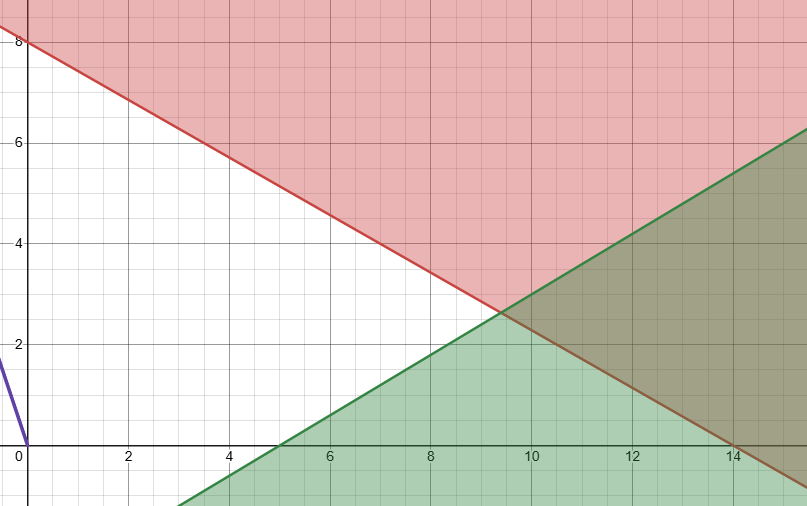
\includegraphics[width=0.7\textwidth]{pic/5-b.png}
\end{figure}


\section{}

求出下面系统中的三个基本解:
\[\begin{aligned}
    x_1 + x_2 + 3 x_3 - x_4 + x_5 &= 4\\
    -x_1 + x_2 - 3 x_3+ 2x_4 - x_5 &= -5
\end{aligned}\]

\paragraph{解,其一} 以x1,x2 为主元 该方程化简为

\[
\begin{bmatrix}
1 &   & 3 & -\frac{5}{3} & 1 &  \\
  & 1 &   & \frac{1}{3} &   & 
\end{bmatrix}
\left[\begin{array}{c} x_1 \\ x_2 \\ x_3 \\ x_4 \\x_5 \end{array}\right] =
\left[\begin{array}{c} \frac{14}{3} \\ -\frac{1}{3} \end{array}\right]
\]

使 $x_3= x_4 = x_5 = 0$,得 $x_1 = \frac{14}{3}, x_2 = -\frac{1}{3}$.



\paragraph{解,其二} 以x1,x4 为主元 该方程写为
\[\begin{aligned}
    x_1  - x_4+ x_2 + 3 x_3 + x_5 &= 4\\
    -x_1 + 2x_4 + x_2 - 3 x_3 - x_5 &= -5
\end{aligned}\]

化简为:

\[
\begin{bmatrix}
1 &   & 5 & 3 & 1 & 13 \\
  & 1 & 3 &   &   & 9
\end{bmatrix}
\left[\begin{array}{c} x_1 \\ x_4 \\ x_2 \\ x_3 \\x_5 \end{array}\right] =
\left[\begin{array}{c} 13 \\ -9\end{array}\right]
\]

使 $x_2= x_3 = x_5 = 0$,得 $x_1 = 13, x_4 = -9$.
\paragraph{解,其三} 以x2,x3 为主元 该方程写为
\[\begin{aligned}
   2x_2 + 3 x_3+ x_1 - x_4  + x_5 &= 4\\
     x_2 - 3 x_3-x_1 + 2x_4 + - x_5 &= -5
\end{aligned}\]

化简为:
\[
\begin{bmatrix}
1 & 3 & 1 & -\frac{4}{3} & 1 \\
  & 1 & \frac{1}{3} & -\frac{5}{9} & \frac{1}{3}  
\end{bmatrix}
\left[\begin{array}{c} x_2 \\ x_3 \\ x_1 \\ x_4 \\x_5 \end{array}\right] =
\left[\begin{array}{c} 1 \\ -\frac{2}{3}\end{array}\right]
\]

令 $x_1,x_4,x_5 = 0$,得 $x_2 = 1, x_3 = -\frac{2}{3}$

\section{}
找出方程 $Ax = b$ 的两个基本解,并指出每个解中的 $B$, $B^{-1}$, $N$,$x_B$, $x_N$.

\[ A = \left[\begin{array}{cccc} 2,4,2,2 \\ 4,10,6,8\end{array}\right], b = \left[\begin{array}{c}4 \\ 12\end{array}\right]
\]
\paragraph{解, 其一}
\[
\left[\begin{array}{cccc}
    1 &2& 1& 1\\
    2& 5& 3 & 4\\
\end{array}\right]
\left[\begin{array}{c} x_1 \\ x_2 \\ x_3 \\ x_4  \end{array}\right] =
\left[\begin{array}{c} 2\\ 6\end{array}\right]
\]
\[
\left[\begin{array}{cccc}
    1 &2& 1& 1\\
     & 1& 1 & 2\\
\end{array}\right]
\left[\begin{array}{c} x_1 \\ x_2 \\ x_3 \\ x_4  \end{array}\right] =
\left[\begin{array}{c} 2\\ 2\end{array}\right]
\]
\[
\left[\begin{array}{cccc}
    1 & & -1& -3\\
     & 1& 1 & 2\\
\end{array}\right]
\left[\begin{array}{c} x_1 \\ x_2 \\ x_3 \\ x_4  \end{array}\right] =
\left[\begin{array}{c} -2\\ 2\end{array}\right]
\]

此时 $B = \begin{bmatrix}
    1 & \\
      & 1
\end{bmatrix}$, $B^{-1} = B$, $N = \begin{bmatrix}
    -1 & -3 \\
    1 & 2
\end{bmatrix}$, $x_B = (x1,x2)^T$, $x_N = (x3,x4)^T$

固定$x_3,x_4$为0,有
\[
\begin{bmatrix}
    1 &  \\
     & 1 \\
\end{bmatrix}
\left[\begin{array}{c} x_1 \\ x_2  \end{array}\right] =
\left[\begin{array}{c} -2\\ 2\end{array}\right]
\]

得 $x_1 = -2, x_2 = 2$, 此时 $x_3 = x_4 = 0$

\paragraph{解, 其二}

这次取$x_1,x_3$进行化简
\[
\left[\begin{array}{cccc}
    1 &2& 1& 1\\
    2& 3& 5 & 4\\
\end{array}\right]
\left[\begin{array}{c} x_1 \\ x_3 \\ x_2 \\ x_4  \end{array}\right] =
\left[\begin{array}{c} 2\\ 6\end{array}\right]
\]
\[
\left[\begin{array}{cccc}
    1 &1& 2& 1\\
     & 1& 1 & 2\\
\end{array}\right]
\left[\begin{array}{c} x_1 \\ x_3 \\ x_2 \\ x_4  \end{array}\right] =
\left[\begin{array}{c} 2\\ 2\end{array}\right]
\]
\[
\left[\begin{array}{cccc}
    1 & & -1& -1\\
     & 1& 1 & 2\\
\end{array}\right]
\left[\begin{array}{c} x_1 \\ x_3 \\ x_2 \\ x_4  \end{array}\right] =
\left[\begin{array}{c} 0\\ 2\end{array}\right]
\]

此时 $B = \begin{bmatrix}
    1 & \\
      & 1
\end{bmatrix}$, $B^{-1} = B$, $N = \begin{bmatrix}
    1 & -1 \\
    1 & 2
\end{bmatrix}$, $x_B = (x1,x3)^T$, $x_N = (x2,x4)^T$

固定$x_3,x_4$为0,有
\[
\left[\begin{array}{cc}
    1 &  \\
     & 1 \\
\end{array}\right]
\left[\begin{array}{c} x_1 \\ x_2  \end{array}\right] =
\left[\begin{array}{c} 0\\ 2\end{array}\right]
\]

得 $x_1 = 0, x_3 = 2$,此时 $x_2 = x_4 = 0$

\section{}

证明:线性规划(LP)问题可行解$x$为基本可行解的充要条件是$x$中正分量对应矩阵$A$的系
数列向量线性无关.


\begin{proof}[充分性]
设 解共有n个变量,其中有m个, $x_1 ... x_m >0$, 而 $x_{m+1} ... x_n = 0$

那么由约束条件 
\[ A \begin{bmatrix}
    x_1 \\ \vdots \\x_m \\ x_{m+1} \\ \vdots \\ x_n
\end{bmatrix} = b\] 

可以得到
\[ \begin{bmatrix} A_1 & A_{r} \end{bmatrix} \begin{bmatrix}
    x_1 \\ \vdots \\x_m \\ 0 \\ \vdots \\ 0
\end{bmatrix} = b\] 

\[  A_1 \begin{bmatrix}
    x_1 \\ \vdots \\x_m 
\end{bmatrix} = b\] 

又 $A_1$中得各列向量线性无关,因此该方程的解是唯一的, 不可能有另一组解$x_1' ... x_m'$.其中含有更多的0.
因此 $(x_1 ,..., x_m, ... ,x_n)$ 是原方程的基本解.

\end{proof}

\begin{proof}[必要性]
\[ \begin{bmatrix} A_1&  A_2\end{bmatrix} \begin{bmatrix}
    x_1 \\ \vdots \\x_m \\ x_{m+1} \\ \vdots \\ x_n
\end{bmatrix} = b\] 

可以化简为 
\[ \begin{bmatrix} I &  A_3\end{bmatrix} \begin{bmatrix}
    x_1 \\ \vdots \\x_m \\ x_{m+1} \\ \vdots \\ x_n
\end{bmatrix} = \begin{bmatrix}
    x_1 \\ \vdots \\ x_m
\end{bmatrix}\] 
即说明 $\begin{bmatrix} A_1&  A_2\end{bmatrix}$ 与$ \begin{bmatrix} I &  A_3\end{bmatrix}$ 等秩, $A_1$ 与 $I$等秩,即它的列向量均线性无关.
\end{proof}

\section{}

用单纯形法求解下列问题
\begin{enumerate}[a)]
    \item Max $z = 6x_1  +14x_2  + 13x_3 s.t. \left\{ \begin{aligned}
        x_1 + 4x_2 + 2x_3  \leq 48 \\
        x_1 + 2x_2 + 4x_3 \leq 60\\
        x_1 , x_2 , x_3 \geq 0
    \end{aligned}\right.$
    \item Min $z = 3x_1 - 2x_2  -4x_3 s.t. \left\{ \begin{aligned}
        4x_1 + 5x_2 - 2x_3  \leq 22 \\
        x_1 - 2x_2 + x_3 \leq 30\\
        x_1 , x_2 , x_3 \geq 0
    \end{aligned}\right.$
    \item Max $z = x_1 +x_2  +x_3 s.t. \left\{ \begin{aligned}
        x_1 + - 2x_3  \leq 5 \\
        2x_1 - 3x_2 + x_3 \leq 3\\
        2x_1 - 5x_2 + 6x_3 \leq 5\\
        x_1 , x_2 , x_3 \geq 0
    \end{aligned}\right.$
\end{enumerate}
    
\paragraph{a}

转换为标准型:

Min \(z=-6x_1-14x_2-13x_3 , s.t. \left\{\begin{aligned}
  x_1+4x_2+2x_3+x_4=48 \\
  x_1+2x_2+4x_3+x_5=60 \\
x_1 ... x_5 \geq 0
\end{aligned}\right.\)

以 $x_1,x_2$为主元,题目化为

\[
\begin{bmatrix}
1 &   & 6 & -1 & 2 \\
  & 1 & -1 & \frac{1}{2} & -\frac{1}{2}
\end{bmatrix} 
\begin{bmatrix}
    x_1 \\ x_2 \\ x_3 \\ x_4 \\ x_5
\end{bmatrix} 
= \begin{bmatrix}
    72 \\ -6
\end{bmatrix}
\]
 
$x_5 = -6 < 0 $ 不符合约束.



以 $x_2,x_5$为主元,题目化为
\[
\begin{bmatrix}
1 &   & \frac{1}{4} & \frac{1}{2} & \frac{1}{4} & 12 \\
  & 1 & \frac{1}{2} & 3 & -\frac{1}{2} & 36
\end{bmatrix}
\begin{bmatrix}
    x_2 \\ x_5 \\ x_1 \\ x_3 \\ x_4
\end{bmatrix} 
= \begin{bmatrix}
    72 \\ -6
\end{bmatrix}
\]
得 $x_2 = 72, x_5 = 6, x_1 = x_3 = x_4 = 0$,此时 $z = -14 * 72 = -1008$

考察其他的组合,分别是$x_1x_5, x_3x_5, x_4 x_5, x_2x_3,x_2x_4$,之前$x_1x_2$为主元已经被判定为不符合要求.

考察$x_1x_5$为主元:

\[
\begin{bmatrix}
1 &   & 4 & 2 & 1\\
  & 1 & -2 & 2 & -1
\end{bmatrix}
\begin{bmatrix}
    x_1 \\ x_5 \\ x_2 \\ x_3 \\ x_4
\end{bmatrix} 
= \begin{bmatrix}
   48 \\ 12
\end{bmatrix}
\]

得 $x_2 = 48, x_5 = 12, x_2 = x_3 = x_4 = 0$,此时 $z = -14 * 48 = -672$,说明 $x_1x_5$不比$x_2x_5$基更好.


考察 $x_3x_5$

\[
\begin{bmatrix}
1 &   & \frac{1}{2} & 2 & \frac{1}{2}  \\
  & 1 & -1 & -6 & -2 
\end{bmatrix}
\begin{bmatrix}
    x_3 \\ x_5 \\ x_1 \\ x_2 \\ x_4
\end{bmatrix} 
= \begin{bmatrix}
  24 \\- 36
\end{bmatrix}
\]

不符合约束.


考察 $x_4x_5$
\[
\begin{bmatrix}
1 &   & 1 & 4 & 2 & 48 \\
  & 1 & 1 & 2 & 4 & 60
\end{bmatrix}
\begin{bmatrix}
    x_4 \\ x_5 \\ x_1 \\ x_2 \\ x_3
\end{bmatrix} 
= \begin{bmatrix}
  48 \\ 60
\end{bmatrix}
\]

此时$z = 0$,不比 $x_2 x_5$ 更好.

考察 $x_1x_5$
\[
\begin{bmatrix}
1 &   & 4 & 2 & 1 \\
  & 1 & -2 & 2 & -1
\end{bmatrix}
\begin{bmatrix}
    x_1 \\ x_5 \\ x_2 \\ x_3 \\ x_4
\end{bmatrix} 
= \begin{bmatrix}
  48 \\ 12
\end{bmatrix}
\]
此时 $x_1 = 48,x_5 = 12$,$z = -6 * 48 = -288 $, 不如$x_2x_5$.

考察 $x_2x_3$
\[
\begin{bmatrix}
1 &   & \frac{1}{6} & \frac{1}{3} & -\frac{1}{6}  \\
  & 1 & \frac{1}{6} & -\frac{1}{6} & \frac{1}{3} 
\end{bmatrix}
\begin{bmatrix}
    x_2 \\ x_3 \\ x_1 \\ x_4 \\ x_5
\end{bmatrix} 
= \begin{bmatrix}
  6 \\ 12
\end{bmatrix}
\]

此时 $ x_2 = 6,x_3 = 12$, $z = -6*14  - 12 * 13 = -240$,不如 $x_2x_5$.

考察 $x_2x_4$
\[
\begin{bmatrix}
1 &   & \frac{1}{2} & 2 & \frac{1}{2} \\
  & 1 & -1 & -6 & -2 
\end{bmatrix}
\begin{bmatrix}
    x_2 \\ x_4 \\ x_1 \\ x_3 \\ x_5
\end{bmatrix} 
= \begin{bmatrix}
  30 \\ -72
\end{bmatrix}
\]
不符合约束.

综上, 得 $x_2 = 72, x_5 = 6, x_1 = x_3 = x_4 = 0$ 是最优解 ,此时 $z = -14 * 72 = -1008$
\paragraph{b}

转换为标准型:

Min \(z=-3x_1+2x_2+4x_3 , s.t. \left\{\begin{aligned}
  4x_1+5x_2-2x_3+x_4=22 \\
  x_1-2x_2+x_3+x_5=30 \\
x_1 ... x_5 \geq 0
\end{aligned}\right.\)

以 $x_2x_3$为主元,

\[
\begin{bmatrix}
1 &   & 6 & 1 & 2 & 82 \\
  & 1 & 13 & 2 & 5 & 194
\end{bmatrix}
\begin{bmatrix}
    x_2 \\ x_3 \\ x_1 \\ x_4 \\ x_5
\end{bmatrix} 
= \begin{bmatrix}
  82 \\ 194
\end{bmatrix}
\]

得 $x_2 = 82,x_3 = 194$, 此时 $z = - 82 * 2 - 194 * 3 = -746$,观察到$x_1$系数为正,它的最好取值即为0,而 $x_4,x_5$ 不改变结果因此 $x_2x_3$就是最好的基元素. 

\paragraph{c}
转换为标准型:

Min \(z=-x_1-x_2-x_3 , s.t. \left\{\begin{aligned}
  x_1-2x_3+x_4=5 \\
  2x_1-3x_2+x_3+x_5=3 \\
  2x_1-5x_2+6x_3+x_6=5 \\
x_1 ... x_6 \geq 0
\end{aligned}\right.\)

经测试, $x_1x_2x_3$ 和 $x_4x_5x_6$是唯二有可行解的基元素选取方式. 

考察 $x_1x_2x_3$,此时问题转化为:

此时问题转化为:
\[
\begin{bmatrix}
1 &   &   & \frac{13}{5} & -2 & \frac{6}{5}  \\
  & 1 &   & 2 & -2 & 1 \\
  &   & 1 & \frac{4}{5} & -1 & \frac{3}{5} 
\end{bmatrix}
\begin{bmatrix}
    x_1 \\ \vdots \\ x_6
\end{bmatrix} 
= \begin{bmatrix}
 13 \\ 9 \\ 4
\end{bmatrix}
\]

此时 $x_1 = 13 , x_2 = 9 x_3 = 4$ ,$z = -13-9-4 = -26$.

考察 $x_4x_5x_6$,此时问题转化为:

此时问题转化为:
\[
\begin{bmatrix}
1 &   &   & 1 &   & -2 \\
  & 1 &   & 2 & -3 & 1 \\
  &   & 1 & 2 & -5 & 6 
\end{bmatrix}
\begin{bmatrix}
    x_4 \\  x_5 \\ x_6 \\ x_1 \\ x_2 \\ x_3
\end{bmatrix} 
= \begin{bmatrix}
 5 \\ 3\\ 5
\end{bmatrix}
\]


此时 $x_4 = 5 , x_5 = 3 x_6 = 5, x_1 = x_2 = x_3 = 0$ ,$z = 0$.


综上, $x_1x_2x_3$ 是最佳的基元素选取方案,此时 $x_1 = 13 , x_2 = 9 x_3 = 4$ ,$z = -13-9-4 = -26$.
\section{}
采用大M法和两段法求解下列问题:

\[\text{Max}\quad 4x_1 + 2x_2 + 8x_3, s.t. \left\{\begin{aligned}
    2x_1 - x_2 + 3x_3 \leq 30 \\
    x_1 + 2x_2 + 4x_3 = 40\\
    x_1,x_2,x_3 \geq 0
\end{aligned}\right.\]

\paragraph{解}
   将问题转化为标准型:

Min \(z=-4x_1-2x_2-8x_3 , s.t. \left\{\begin{aligned}
  2x_1-x_2+3x_3+x_4=30 \\
  x_1+2x_2+4x_3=40 \\
x_1  ... x_4 \geq 0
\end{aligned}\right.\)

\paragraph{大M法}

新增变量 \(x_5\),与\(x_4\)构成单位矩阵. 此时问题为 :

Min \(z=-4x_1-2x_2-8x_3 + Mx_5 , s.t. \left\{\begin{aligned}
  2x_1-x_2+3x_3+x_4=30 \\
  x_1+2x_2+4x_3 + x_5=40 \\
x_1  ... x_5 \geq 0
\end{aligned}\right.\)

此时的初始解为 $x_4 = 30, x_5 = 40, x_1,x_2,x_3 = 0$. 经过多轮迭代之后:

取 $x_1x_2$ 为基元素,原问题化解为:

\[
\begin{bmatrix}
1 &   & 2 & \frac{2}{5} & \frac{1}{5}  \\
  & 1 & 1 & -\frac{1}{5} & \frac{2}{5} 
\end{bmatrix}
\begin{bmatrix}
    x_1 \\ \vdots \\  x_5
\end{bmatrix} 
\begin{bmatrix}
    20 \\ 10
\end{bmatrix} 
\]

此时 $x_1 = 20, x_2 = 10, x_3=x_4 = x_5 = 0$,对应原问题的解为 $x_1 = 20, x_2 = 10, x_3 = 0$, 此时 $z = 4 * 20 + 2 * 10 = 100$.


\paragraph{二阶段法}

% 第一阶段\footnote{参考 https://zhuanlan.zhihu.com/p/266266080}: 新增变量 \(\),与\(x_4\)构成单位矩阵, 此时问题为 :


Min \(z=x_5 , s.t. \left\{\begin{aligned}
  2x_1-x_2+3x_3+x_4=30 \\
  x_1+2x_2+4x_3 + x_5=40 \\
x_1  ... x_5 \geq 0
\end{aligned}\right.\)

此时的初始解为 $x_4 = 30, x_5 = 40, x_1,x_2,x_3 = 0$. 经过多轮迭代之后,得到$x_2x_3$可以作为基元素.此时问题转化为

\[
\begin{bmatrix}
1 &   & 1 & -\frac{1}{5} & \frac{2}{5}\\
  & 1 & -2 & \frac{4}{5} & -\frac{3}{5} 
\end{bmatrix}
\begin{bmatrix}
    x_2 \\ x_3 \\ x_1 \\ x_4 \\  x_5
\end{bmatrix} 
\begin{bmatrix}
    10 \\ 0
\end{bmatrix} 
\]


第二阶段: 从 $x_2,x_3$ 开始迭代,直到发现$x_1x_2$为最好的基元素. 此时 $x_1 = 20, x_2 = 10, x_3=x_4 = x_5 = 0$,对应原问题的解为 $x_1 = 20, x_2 = 10, x_3 = 0$, 此时 $z = 4 * 20 + 2 * 10 = 100$.
\section{}

证明:线性规划问题的对偶问题的对偶问题是原问题.\footnote{参考 https://zhuanlan.zhihu.com/p/259516554}

\begin{proof}
设原问题为

\[\text{Max}\quad z = \sum_{j=1}^n c_jx_j, s.t. \left\{\begin{aligned}
    \sum_{j=1}^n a_ij x_j \leq b_i, \quad (i = 1 ... m) \\
    x_j \geq 0 \quad (j = 1 ... n)
\end{aligned}\right.\]

其对偶问题为:
\[\text{Min}\quad z = \sum_{i=1}^m b_iy_i, s.t. \left\{\begin{aligned}
    \sum_{i=1}^m a_ij y_i \leq c_i, \quad (j = 1 ... n) \\
    y_i \geq 0 \quad (i = 1 ... m)
\end{aligned}\right.\]

由定义写出对偶问题的对偶问题:

\[\text{Max}\quad z = \sum_{j=1}^n c_jx_j, s.t. \left\{\begin{aligned}
    \sum_{j=1}^n a_ij x_j \leq b_i, \quad (i = 1 ... m) \\
    x_j \geq 0 \quad (j = 1 ... n)
\end{aligned}\right.\]

\end{proof}


\section{}
讨论线性规划问题与其对偶问题的联系与区别。
\paragraph{答}

线性规划问题与其对偶问题之间存在紧密的联系与显著的区别。每个线性规划问题都有一个对应的对偶问题,原问题称为“Primal”,而对偶问题称为“Dual”。这两者之间的关系体现在多个方面:首先,弱对偶性保证了如果原问题有可行解,则对偶问题的目标函数值不超过原问题的目标函数值。其次,在满足强对偶性的条件下(例如Slater条件),原问题的最优值等于对偶问题的最优值。

在结构上,原问题通常是最大化目标函数,约束条件为线性不等式,而对偶问题则是最小化目标函数,其约束条件与原问题相对应。变量的意义也有所不同:原问题的变量代表决策水平(如生产量),而对偶问题的变量通常表示对约束的影子价格或资源的价值。

理解线性规划的对偶性不仅有助于求解优化问题,还在经济学中提供了资源分配的深刻见解。通过对原问题和对偶问题的比较,优化者可以获得更全面的决策依据。

\section{}
判断下列说法是否正确:
\begin{enumerate}[a)]
    \item 考虑具有有界可行集的线性规划问题,如果是$x$一个最优解,则其必定是一个最优
基本可行解。 \textcolor{green}{对}
\item 如果线性规划问题有多个解,则其必定有无穷多个解。 \textcolor{green}{对 此时说明可行域是无限大的,且目标函数的梯度没有与某个限定条件相反.}
\item 考虑标准形式的线性规划问题:$min c^Tx, s. t. Ax = b, x \geq 0$,这里矩阵A的维数为$m \times n$,且行满秩。每个最优解上最多有个$m$变量值为正。\textcolor{green}{对}
\item 对于(c)中的标准线性规划问题,可行域的每个顶点至多有$n-m$个相邻顶点。\textcolor{red}{错}
\end{enumerate}

\section{}

总结线性规划的单纯性方法的基本流程,尝试编程序写出该方法的实现,并以上面的任
意例子为例,给出运行结果。

见 https://github.com/HOMODELUNA/convex-optimizations

\section{}
请安装 Julia,安装 MWorks 科教版(或者安装 JuMP 包)。使用里面的凸优化工具箱。然
后尝试调用里面的求解器求解第 2 章中的制作 100 套钢管的例题。

见 https://github.com/HOMODELUNA/convex-optimizations
\section{}

请辨析:线性优化与非线性优化,凸优化与非凸优化,光滑优化与非光滑优化之间的区
别和联系,并简要介绍如何进行线性化、凸化和光滑化。以及为什么凸优化与非凸优化
的分析是目前的主流。

\paragraph{答}

\begin{table}[H]
    \centering
    \begin{tabular}{lll}
         & 线性优化 & 非线性优化 \\
        目标函数或约束条件 & 都是线性 & 至少有一个不是线性 \\
        求解方法 & 多,单纯形法,内点法 & 梯度法,牛顿法 
    \end{tabular}
\end{table}
\begin{table}[H]
    \centering
    \begin{tabular}{lll}
         & 凸优化 & 非凸优化 \\
        目标函数或可行域 & 凸函数,凸集 & 至少有一个不是凸 \\
        解的性质 & 局部最优解就是全局最优解 & 可能有多个局部最优解
    \end{tabular}
\end{table}

\textbf{光滑优化}:目标函数在可行域内是可微的,具有良好的导数性质,便于应用传统的优化算法(如梯度法)。

\textbf{非光滑优化}:目标函数可能在某些点不可微,需使用次梯度法等方法处理。非光滑问题更常见于实际应用,如L1正则化。

线性化:将非线性问题近似为线性问题,通常通过泰勒展开在某个点处进行线性化。
例如,针对函数 $f(x)$, 在 $x_0$ 附近的线性化为:
$ f(x) = f(x_0) + f'(x_0)(x-x_0) $

凸化: 将非凸问题转化为凸问题,可能通过引入新的变量、约束或使用松弛技术。例如使用凸包或增加约束来限制可行域。

光滑化:将非光滑函数转化为光滑函数,常通过正则化技术(如添加平滑项)实现。
例如,使用  $L_2$正则化替代 $L_1$正则化,使目标函数光滑。

凸优化的分析是主流,原因包括:
\begin{itemize}
    \item 理论基础:凸优化有丰富的数学理论,提供了强大的工具和方法来证明收敛性和最优性。
    \item 计算效率:凸问题的求解普遍比非凸问题更高效,且在众多实际应用中能够找到全局最优解。
    \item 广泛应用:许多实际问题可以通过适当的变换转化为凸优化问题,从而利用其优势。
\end{itemize}


\section{}

请介绍线性规划内点法的核心思想。

\paragraph{答}

线性规划内点法是一种求解线性规划问题的有效算法,其核心思想主要包括以下几个方面:

\begin{itemize}
    \item 可行区域的内部:与传统的单纯形法不同,内点法在可行解的内部进行搜索,而不是沿着边界。这允许算法在每一步中保持在可行区域内。
    \item 中心路径:算法通过跟踪一个被称为“中心路径”的轨迹来逐步接近最优解。这个路径由一系列点组成,这些点不仅满足约束条件,同时也尽量使目标函数的值达到最优。
    \item 障碍函数:内点法通常引入一个障碍函数,防止搜索路径靠近可行域的边界。这种函数会在靠近边界时增加目标函数的值,从而引导算法保持在内部。
    \item 迭代更新:算法通过迭代更新当前解,每一步都会计算一个新的解,通常使用牛顿法或其他优化技术来加速收敛。
    \item 收敛性:内点法在理论上被证明具有良好的收敛性,通常在多项式时间内找到最优解。这使得内点法在求解大规模线性规划问题时非常有效。
\end{itemize}
Min \(z=-2x_1-1x_2-2x_3+2x_5 , s.t. \left\{\begin{aligned}
  -1x_1-1x_2+1x_3-1x_5=4 \\
  -1x_1-1x_2-1x_3+1x_4+1x_5=6 \\
x_1 \geq 0,x_2 \geq 0,x_3 \geq 0,x_4 \geq 0,x_5 \geq 0
\end{aligned}\right.\)




\end{document}